\section{ارجاع‌دهی‌‌ها}
\begin{frame}{ارجاع‌دهی‌‌ها در خود سند}
\begin{itemize}\itemr
\item[-]
در مواقع زیادی نیاز به ارجاع‌دهی در قسمت‌ها مختلف سند، احساس می‌شود.
\item[-]
برای مثال برای ارجاع‌دهی به یک فصل خاص، سکشن‌ خاص، جدول و یا تصاویر مختلف نیاز به یک ارجاع‌دهی پویا داریم.

\item[-]
فرض کنید چنین متنی داریم: \textit{با توجه به مباحثی که در فصل ۲ انجام شد...}
و سپس تصمیم می‌گیریم که قبل از فصل ۲، یک فصل دیگر بنویسیم و در واقع فصل ۲، می‌شود فصل ۳.

\item[-]
اگر این ارجاع‌دهی را به صورت دستی انجام داده باشیم، باید بگردیم و تمامی \textit{فصل ۲}‌های داخل متنمان را به \textit{فصل ۳} تغییر بدهیم.

\item[-]
اما، همانند کاری که برای شمارنده‌ها کردیم، میتوانیم از امکانات خود لاتک برای ارجاع‌دهی استفاده کنیم.
\end{itemize}
\end{frame}

\begin{frame}{ارجاع‌دهی‌‌ها در خود سند}
\begin{itemize}\itemr
\item[-]
برای اینکار باید از دو دستور استفاده کنیم:
\begin{enumerate}\itemr
\item 
\lr{\texttt{\textbackslash lable\{UniqueLabel\}}} 
برای نشانه‌گذاری

\item 
\lr{\texttt{\textbackslash ref\{UniqueLable\}}}
برای ارجاع‌دهی 
\end{enumerate}
\end{itemize}
\end{frame}

\begin{frame}[fragile]{نمونه کد}
\begin{latin}
\begin{lstlisting}[keywords={chapter, section, label, ref}, keywordstyle=\color{Mulberry}\textbf]
\chapter{Processes and Threads}
\section{Processes}\label{processes}
\section{Threads}
As mentioned in the \ref{processes},
OS must schedule and dispatch...
\end{lstlisting}
\end{latin}
\end{frame}

\begin{frame}{خروجی}
\begin{center}
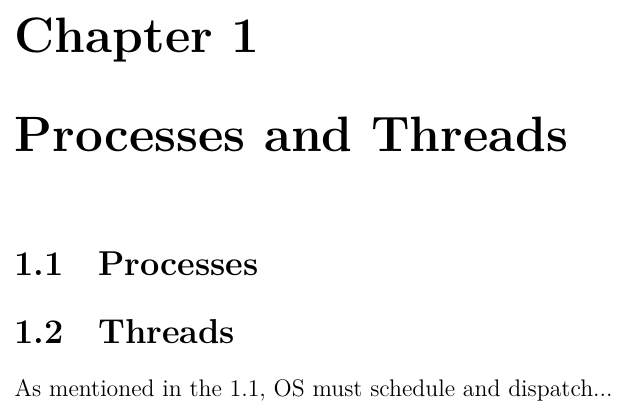
\includegraphics[width=0.65\textwidth, height=0.7\textheight]{docs/images/proc-ref}
\end{center}
\end{frame}


\begin{frame}[fragile]{نمونه کد}
\begin{latin}
\begin{lstlisting}[keywords={chapter, section, label, ref}, keywordstyle=\color{Mulberry}\textbf]
\chapter{Processes and Threads}
\section{Operating System}
\section{Processes}\label{processes}
\section{Threads}
As mentioned in the \ref{processes}, 
OS must schedule and dispatch...
\end{lstlisting}
\end{latin}
\end{frame}

\begin{frame}{خروجی}
\begin{center}
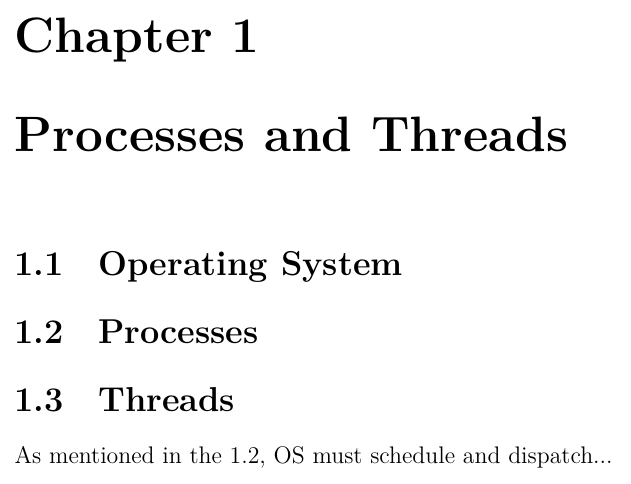
\includegraphics[width=0.55\textwidth, height=0.7\textheight]{docs/images/proc-ref-1}
\end{center}
\end{frame}

\begin{frame}{ارجاع‌دهی‌‌ها در خود سند}
\begin{itemize}\itemr
\item[-]
حتی می‌توان بجای ارجاع‌دهی با عدد، با نام هم به مطلب مورد نظر، ارجاع داد.

\item[-]
برای این کار باید از بسته‌ی 
\lr{\texttt{nameref}}
و تگ
\lr{\texttt{\textbackslash nameref\{UniqueLable\}}}
استفاده کرد.
\end{itemize}
\end{frame}

\begin{frame}[fragile]{نمونه کد}
\begin{latin}
\begin{lstlisting}[keywords={chapter, section, label, ref}, keywordstyle=\color{Mulberry}\textbf]
\chapter{Processes and Threads}
\section{Processes}\label{processes}
\section{Threads}
As mentioned in the \nameref{processes},
OS must schedule and dispatch...
\end{lstlisting}
\end{latin}
\end{frame}

\begin{frame}{خروجی}
\begin{center}
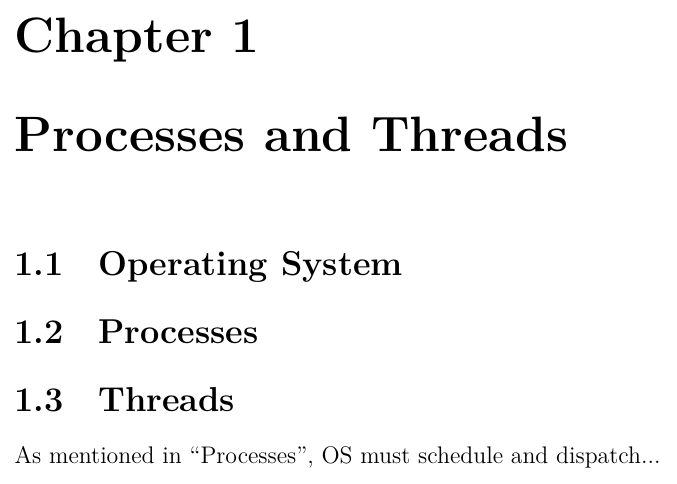
\includegraphics[width=0.55\textwidth, height=0.7\textheight]{docs/images/proc-nameref}
\end{center}
\end{frame}

\begin{frame}[fragile]{نمونه کد}
\begin{latin}
\begin{lstlisting}[keywords={chapter, section, label, ref}, keywordstyle=\color{Mulberry}\textbf]
\chapter{Processes and Threads}
\section{What Are Processes?}\label{processes}
\section{Threads}
As mentioned in the \nameref{processes},
OS must schedule and dispatch...
\end{lstlisting}
\end{latin}
\end{frame}

\begin{frame}{خروجی}
\begin{center}
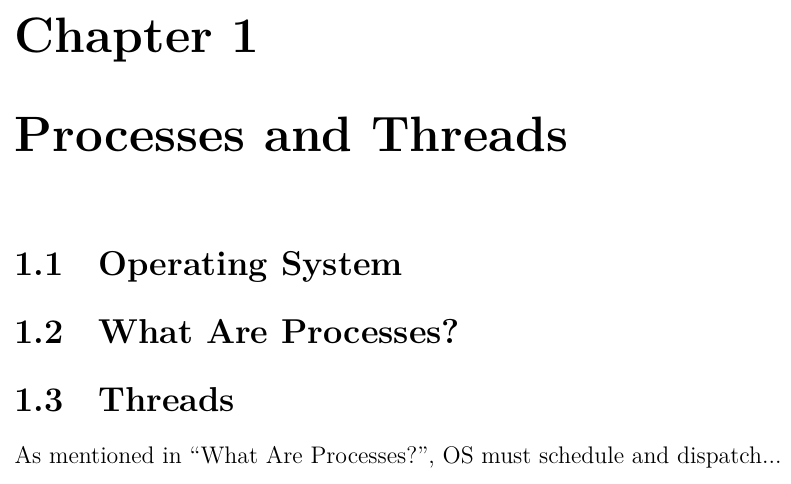
\includegraphics[width=0.7\textwidth, height=0.75\textheight]{docs/images/proc-nameref-change}
\end{center}
\end{frame}

\begin{frame}{فهرست منابع}
\begin{itemize}\itemr
\item[-]
برای یک مقاله یا پایان‌نامه، وجود فهرست منابع کامل و ارجاع به موقع به آنها بسیار ضروری‌ست.

\item[-]
معمولا برای فهرست منابع پایان‌نامه‌ها و مقالات، دانشگاه‌ها و ژورنال‌ها قواعد خاص خود را دارند که در اختیار دانشجویان یا نویسندگان مقاله قرار می‌دهند.
\end{itemize}
\end{frame}

\begin{frame}{فهرست منابع}
\begin{itemize}\itemr
\item[-]
برای یک مقاله یا پایان‌نامه، وجود فهرست منابع کامل و ارجاع به موقع به آنها بسیار ضروری‌ست.

\item[-]
معمولا برای فهرست منابع پایان‌نامه‌ها و مقالات، دانشگاه‌ها و ژورنال‌ها قواعد خاص خود را دارند که در اختیار دانشجویان یا نویسندگان مقاله قرار می‌دهند.
\end{itemize}
\end{frame}

\begin{frame}{استفاده از \lr{Bib\TeX}}
\begin{itemize}\itemr
\item[-]
در این روش، اطلاعات تمامی منابع مورد استفاده با فرمت 
\lr{Bib\TeX}
در یک فایل با پسوند \lr{bib} نوشته می‌شوند.

\item[-]
برای دریافت آن فرمت خاص باید از 
\url{https://scholar.google.com/}
استفاده کرد.
\end{itemize}
\end{frame}

\begin{frame}{جستجوی مقاله}
\begin{center}
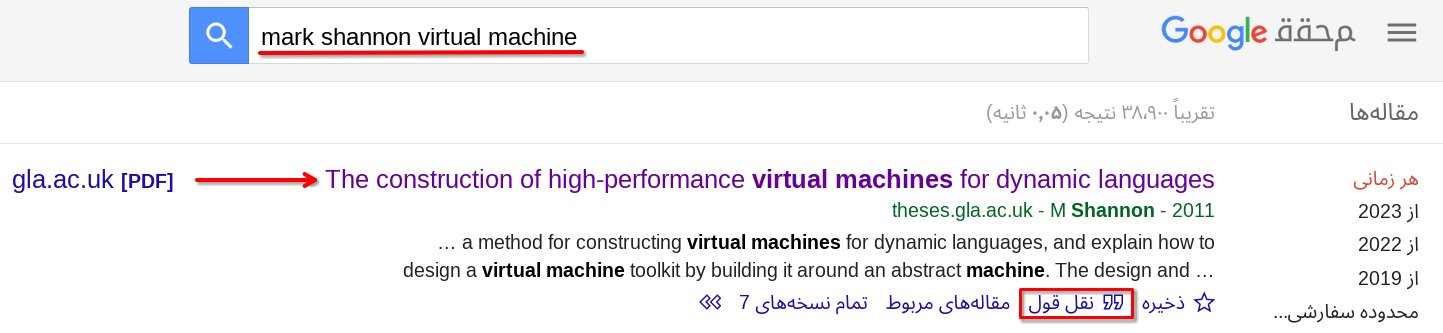
\includegraphics[width=\textwidth]{docs/images/search}
\end{center}
\end{frame}

\begin{frame}{استفاده از \lr{Bib\TeX}}
\begin{center}
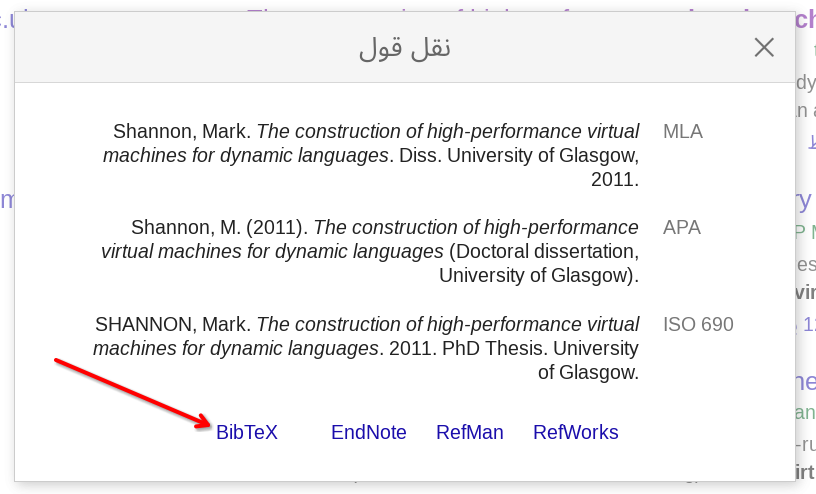
\includegraphics[width=0.8\textwidth, height=0.8\textheight]{docs/images/bibtex}
\end{center}
\end{frame}

\begin{frame}{کپی و ذخیره‌ کردن آن}
\begin{center}
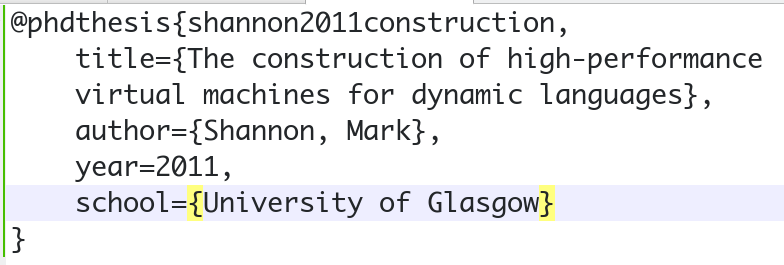
\includegraphics[width=\textwidth]{docs/images/copy-save}
\end{center}
\end{frame}

\begin{frame}[fragile]{فرمت \lr{plain}}
\begin{latin}
\begin{lstlisting}[keywords={chapter, section, label, ref}, keywordstyle=\color{Mulberry}\textbf]
\chapter{Virtual Machines}
In \cite{shannon2011construction}, Dr. Mark Shannon discusses...

\section{Stack Machines}
But also in \cite{shannon2006ac} we disagrees with...

\bibliographystyle{plain}  % HERE
\bibliography{ref}
\end{lstlisting}
\end{latin}
\end{frame}

\begin{frame}{در متن}
\begin{center}

\includegraphics[width=0.55\textwidth, height=0.7\textheight]{docs/images/plain-1}
\end{center}
\end{frame}

\begin{frame}{در فهرست}
\begin{center}

\includegraphics[width=0.9\textwidth, height=0.5\textheight]{docs/images/plain-2}
\end{center}
\end{frame}

\begin{frame}{فرمت \lr{unsrt} در متن}
\begin{center}

\includegraphics[width=0.55\textwidth, height=0.7\textheight]{docs/images/unsrt-1}
\end{center}
\end{frame}

\begin{frame}{فرمت \lr{unsrt} در فهرست}
\begin{center}

\includegraphics[width=0.9\textwidth, height=0.5\textheight]{docs/images/unsrt-2}
\end{center}
\end{frame}

\begin{frame}{فرمت \lr{alpha} در متن}
\begin{center}

\includegraphics[width=0.55\textwidth, height=0.7\textheight]{docs/images/alpha-1}
\end{center}
\end{frame}

\begin{frame}{فرمت \lr{alpha} در فهرست}
\begin{center}

\includegraphics[width=0.9\textwidth, height=0.5\textheight]{docs/images/alpha-2}
\end{center}
\end{frame}

\begin{frame}{فرمت \lr{apalike} در متن}
\begin{center}

\includegraphics[width=0.55\textwidth, height=0.7\textheight]{docs/images/apalike-1}
\end{center}
\end{frame}

\begin{frame}{فرمت \lr{apalike} در فهرست}
\begin{center}

\includegraphics[width=0.9\textwidth, height=0.5\textheight]{docs/images/apalike-2}
\end{center}
\end{frame}

\begin{frame}{فرمت \lr{ieeetr} در متن}
\begin{center}

\includegraphics[width=0.55\textwidth, height=0.7\textheight]{docs/images/ieeetr-1}
\end{center}
\end{frame}

\begin{frame}{فرمت \lr{ieeetr} در فهرست}
\begin{center}

\includegraphics[width=0.9\textwidth, height=0.5\textheight]{docs/images/ieeetr-2}
\end{center}
\end{frame}
